% Niveau :      PCSI
% Discipline :  Mécaflu
%Mots clés :    

\begin{exercise}{Le profil de la tour Eiffel}{1}{Sup, Spé}
{Statique des fluides, Mécanique}{bermu}

\begin{questions}
    \questioncours Redémontrer l'équation de la statique des fluides. 
\begin{EnvUplevel}
Dans ce qui va suivre, on s'intéresse au profil de la tour Eiffel.
\begin{figure}[H]
    \centering
    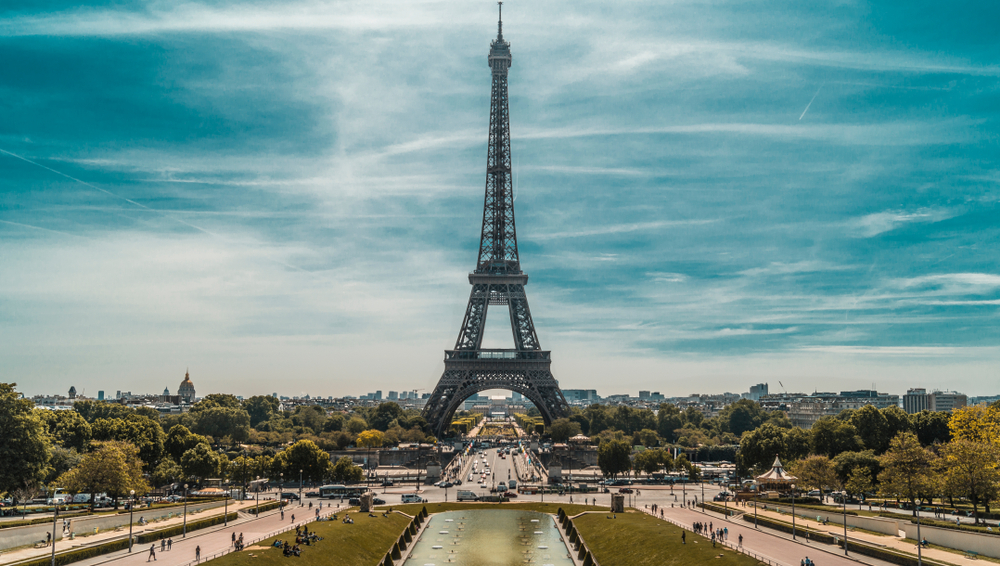
\includegraphics[width=\linewidth]{mecaflu/statiqueflu/eiffel.png}
    \vspace{-1.5em}
    \caption{La tour Eiffel depuis le Trocadéro.}
\end{figure}
\end{EnvUplevel}
    \question Considérant que la structure de la tour Eiffel est conçue afin que chaque étage exerce la même pression sur les étages inférieurs (on pourra discuter de ce principe d'ingénierie civile), établir à l'aide de la figure ci-dessus et des données un modèle simple de la tour Eiffel et donner alors l'équation de son profil.
\end{questions}

\paragraph{Données :}
\begin{itemize}
    \item accélération de la pesanteur terrestre $g = 10$ m$^2\cdot$s$^{-1}$,
    \item masse volumique de l'acier $\rho = 8\cdot 10^3$ $\mathrm{kg\cdot m^{-3}}$,
    \item hauteur de la tour Eiffel $H = 300$ m,
    \item largeur de la base de la tour Eiffel $L = 125$ m.
\end{itemize}
\end{exercise}